\documentclass[11pt]{article}

% ---------------- Packages ----------------
\usepackage[utf8]{inputenc}
\usepackage[T1]{fontenc}
\usepackage{lmodern}
\usepackage{amsmath, amssymb}
\usepackage{graphicx}
\usepackage{float}
\usepackage{hyperref}
\usepackage{booktabs}
\usepackage{caption}
\usepackage{subcaption}
\usepackage{geometry}
\usepackage{appendix}

\geometry{margin=1in}

% ---------------- Title ----------------
\title{FLOWER: A Flow-Matching Solver for Inverse Problems \\[0.3em]
\large Project Report}

\author{Clement Dureuil, Titouan Pottier}

\date{}

% ---------------- Document ----------------
\begin{document}

\maketitle

\section{Introduction}
\noindent
Inverse problems aim to recover an unknown signal $x$ from incomplete and noisy measurements
\begin{equation}
    y = Hx + n,
\end{equation}
where $H$ is the forward operator and $n$ is measurement noise.
Classical methods use hand-crafted regularization, but they can struggle when the true data distribution is complex.
Generative models provide a more expressive prior by learning realistic sample geometry from data.

\medskip
\noindent
In this project, we study \textbf{FLOWER}, a flow-matching based solver for inverse problems.
The method alternates three operations: flow-consistent destination estimation, measurement-driven refinement, and time progression.
This structure explicitly combines a learned generative prior with data fidelity.

\medskip
\noindent
We evaluate the method in two settings:
\begin{enumerate}
    \item a 2D toy inverse problem with a conditional Gaussian mixture model (GMM),
    \item a face image super-resolution task with a pretrained FLOWER model.
\end{enumerate}
The toy setup is used for interpretability and trajectory visualization, while the image setup tests practical reconstruction quality.

\section{Method: FLOWER}
\subsection{Flow-matching prior}
Let $v_{\theta}(x,t)$ be a time-conditioned network that predicts a velocity field.
Starting from Gaussian noise $x_0 \sim \mathcal{N}(0,I)$, samples are transported through
\begin{equation}
    \frac{dx_t}{dt} = v_{\theta}(x_t,t), \quad t \in [0,1].
\end{equation}
In our 2D experiment, $v_{\theta}$ is a time-conditioned MLP implemented in \texttt{scripts/gmm\_flow\_model.py}.
Sampling is done with forward Euler integration.

\subsection{Three-step FLOWER update}
At iteration $k$, with $t_k = k/N$ and current state $x_k$, we apply:

\paragraph{Step 1: destination estimation.}
\begin{equation}
    \hat{x} = x_k + (1-t_k)\,v_{\theta}(x_k,t_k).
\end{equation}
This gives a flow-consistent destination estimate.

\paragraph{Step 2: measurement refinement.}
We enforce consistency with observations by solving
\begin{equation}
    x^\star = \arg\min_x \frac{1}{2\sigma_n^2}\|Hx-y\|_2^2 + \frac{1}{2\lambda_t}\|x-\hat{x}\|_2^2.
\end{equation}
In 2D with linear observation this has a closed-form Gaussian update; for image super-resolution we solve the associated linear system with conjugate gradient (\texttt{cg\_solve} in \texttt{scripts/flower\_steps.py}).

\paragraph{Step 3: time progression.}
\begin{equation}
    x_{k+1} = t_{k+1}x^\star + (1-t_{k+1})z,\quad z\sim\mathcal{N}(0,I).
\end{equation}
This advances the trajectory while keeping the flow schedule.

\medskip
\noindent
The full implementation is provided in \texttt{scripts/flower\_steps.py} for both 2D trajectories and image inverse problems.

\section{Experimental Setup}
\subsection{GMM}
\noindent
We build a 2D inverse problem where the prior is a Gaussian mixture and measurements are noisy linear projections.
The pipeline is:
\begin{enumerate}
    \item generate synthetic prior/posterior data (\texttt{scripts/create\_gmm\_data.py}),
    \item train a flow-matching model on posterior samples (\texttt{scripts/train\_gmm\_flow\_matching.py}),
    \item run FLOWER trajectories and save intermediate states (\texttt{scripts/flower\_steps.py}),
    \item visualize step-by-step dynamics (\texttt{scripts/flower\_plotting.py}).
\end{enumerate}
This setting makes each FLOWER step directly interpretable in 2D.

\subsection{Face images}
\noindent
We consider single-image super-resolution as an inverse problem:
\begin{equation}
    y = Hx + n,
\end{equation}
where $H$ is a downsampling operator and $n$ is additive Gaussian noise.
In our code, local downsampling and its adjoint are implemented in \texttt{scripts/faces\_pipeline.py}.

\medskip
\noindent
We use a pretrained FLOWER model (CelebA setting) from the \texttt{mehrsapo\_Flower/} source folder.
For a custom face image, we:
\begin{enumerate}
    \item generate a noisy low-resolution observation,
    \item reconstruct the high-resolution image with the three FLOWER steps,
    \item compare to simple baselines (adjoint and bicubic interpolation),
    \item evaluate reconstruction quality with PSNR (\texttt{psnr\_torch}).
\end{enumerate}
This experiment checks that the same algorithmic structure scales from an interpretable toy problem to realistic image reconstruction.

\section{Results}
\subsection{GMM: step-by-step behavior}
\noindent
Figure~\ref{fig:gmm_steps} shows the 2D trajectory evolution under the three FLOWER steps.
Qualitatively, Step~1 moves samples toward flow-consistent regions, Step~2 contracts them toward measurement-consistent zones, and Step~3 propagates the process to the next time index while preserving stochasticity.
This confirms the intended decomposition of the algorithm in a fully interpretable setting.

\begin{figure}[H]
    \centering
    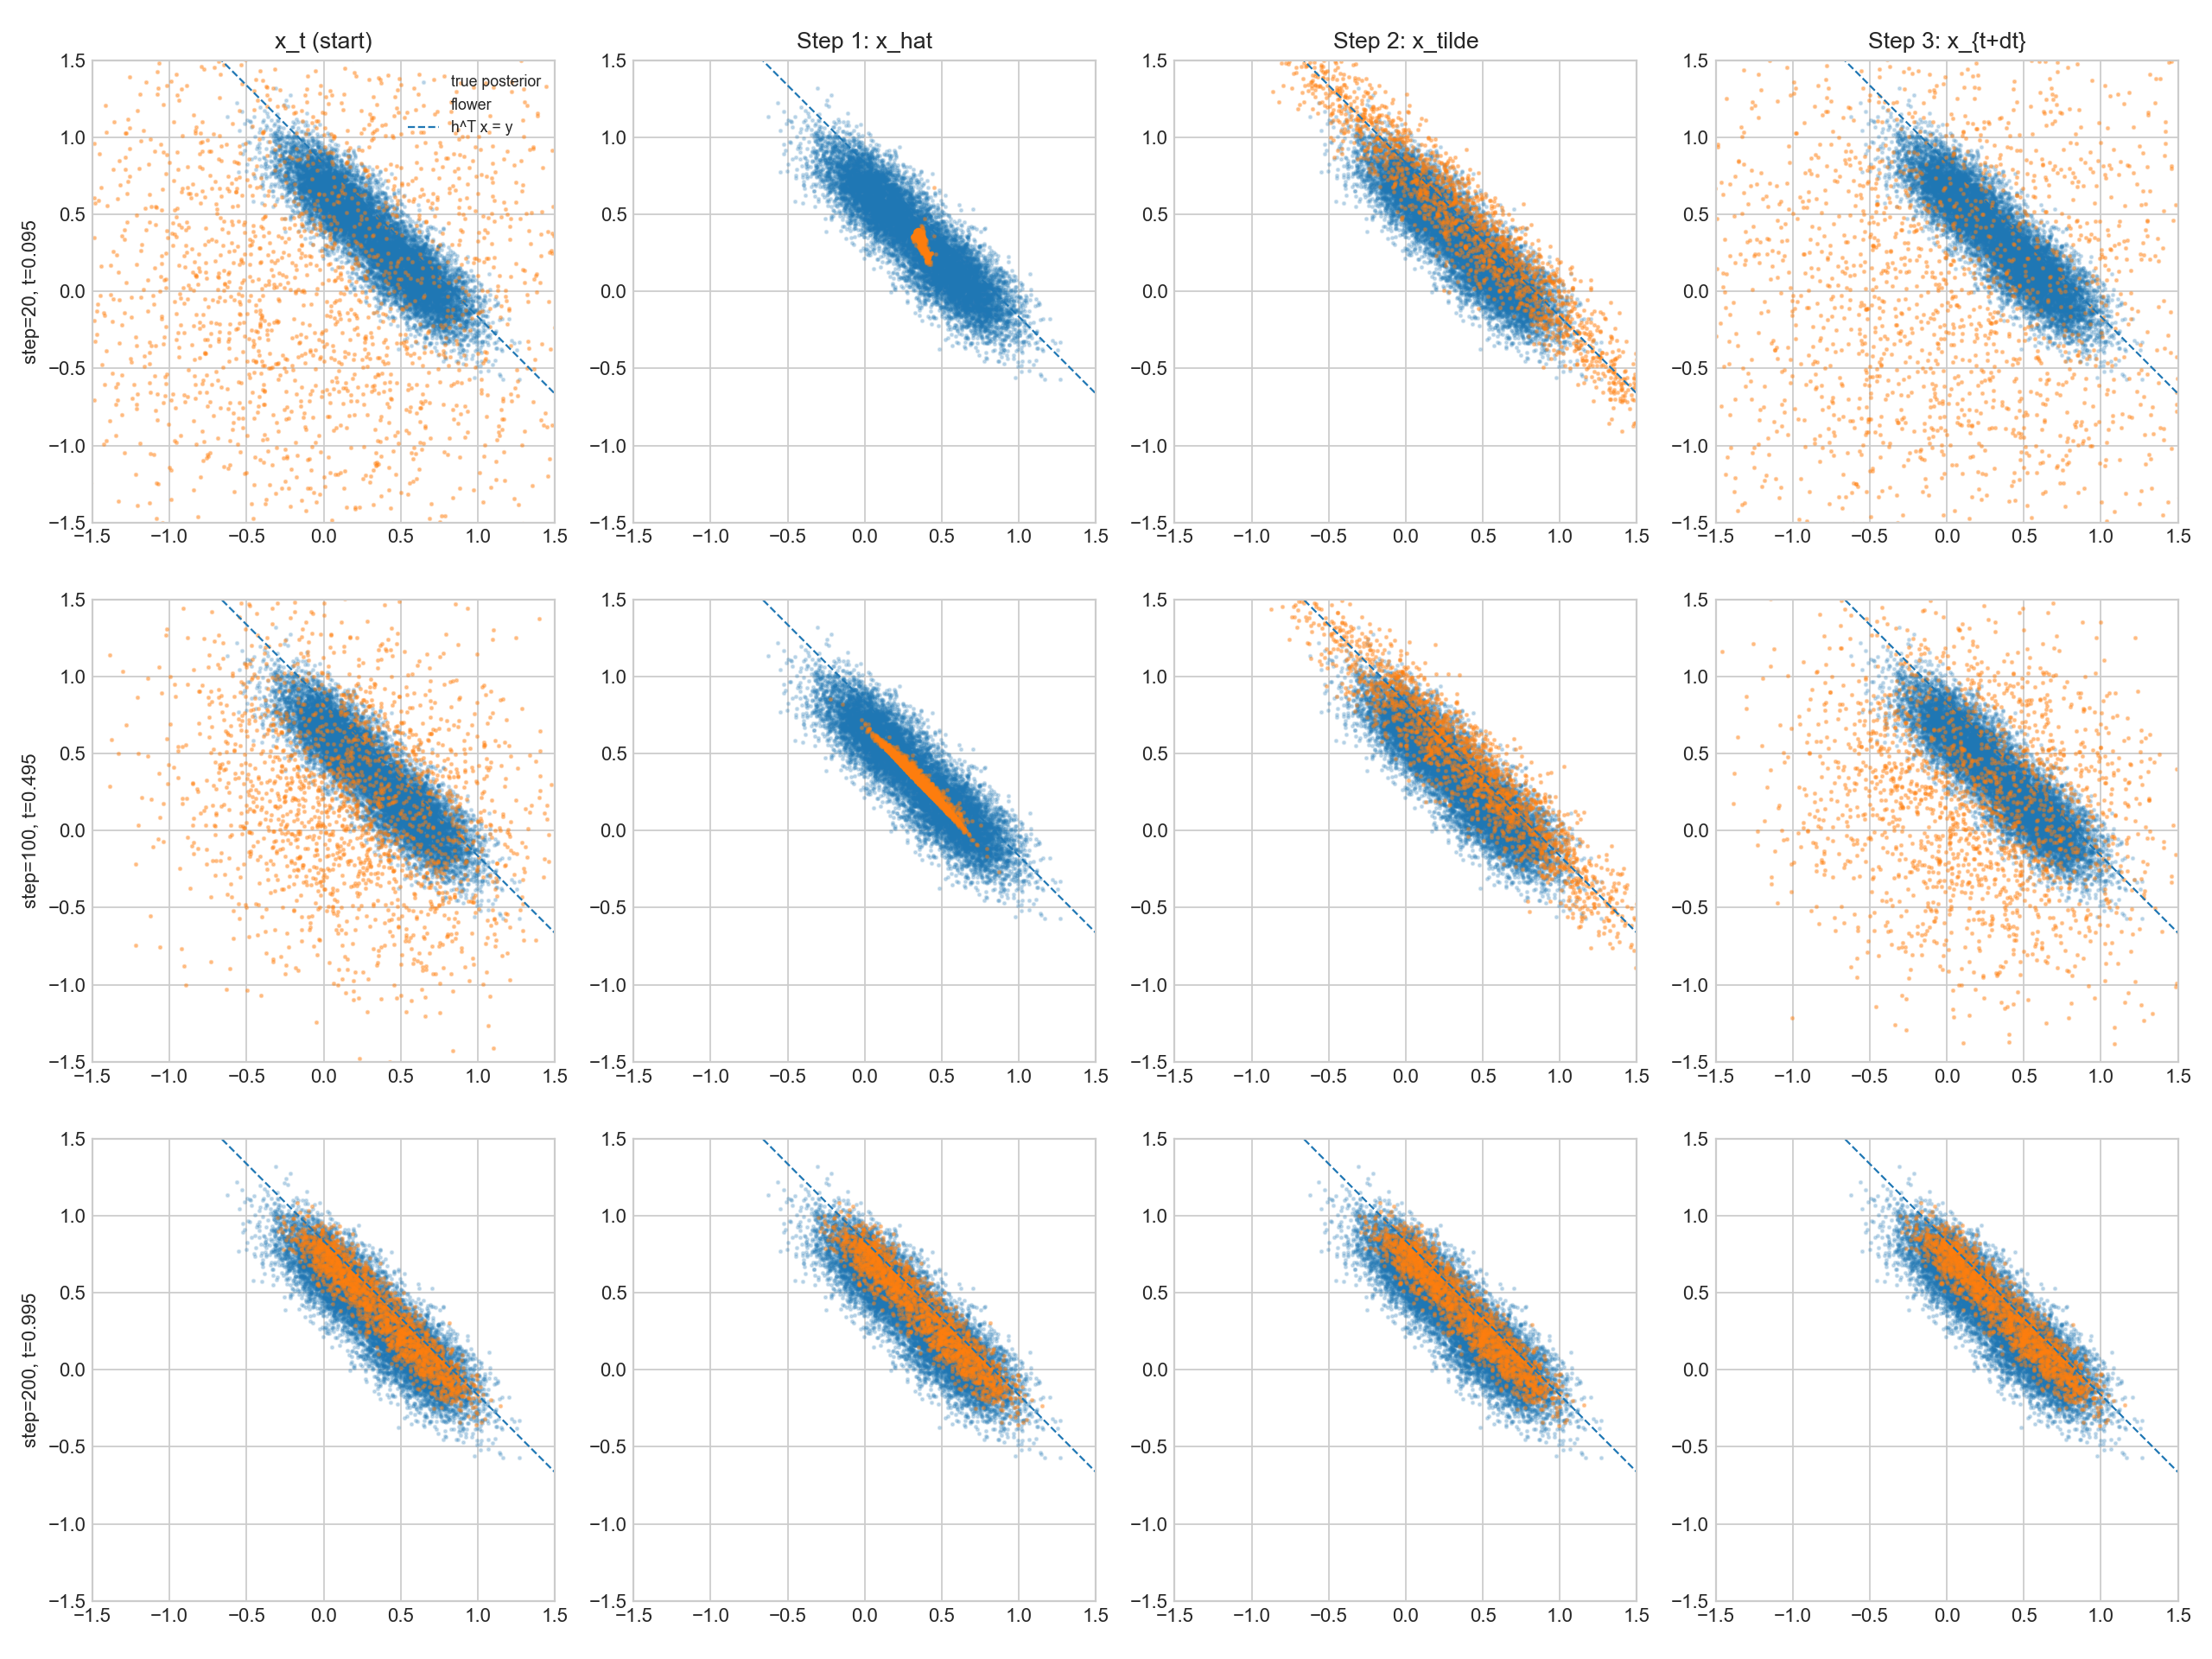
\includegraphics[width=0.92\linewidth]{results_examples/gmm/flower_step_by_step.png}
    \caption{Step-by-step visualization of FLOWER dynamics on the 2D GMM inverse problem.}
    \label{fig:gmm_steps}
\end{figure}

\subsection{Face super-resolution}
\noindent
On face images, the same three-step mechanism produces reconstructions that are visually sharper than direct upsampling baselines.
Figure~\ref{fig:faces_steps} illustrates the reconstruction process and intermediate states, and Figure~\ref{fig:faces_compare} compares final outputs against bicubic interpolation.

\begin{figure}[H]
    \centering
    \begin{subfigure}[t]{0.49\linewidth}
        \centering
        \includegraphics[width=\linewidth]{results_examples/faces/flower_pretrained_superres_steps_dense_with_refs.png}
        \caption{Pretrained model: dense step visualization.}
    \end{subfigure}
    \hfill
    \begin{subfigure}[t]{0.49\linewidth}
        \centering
        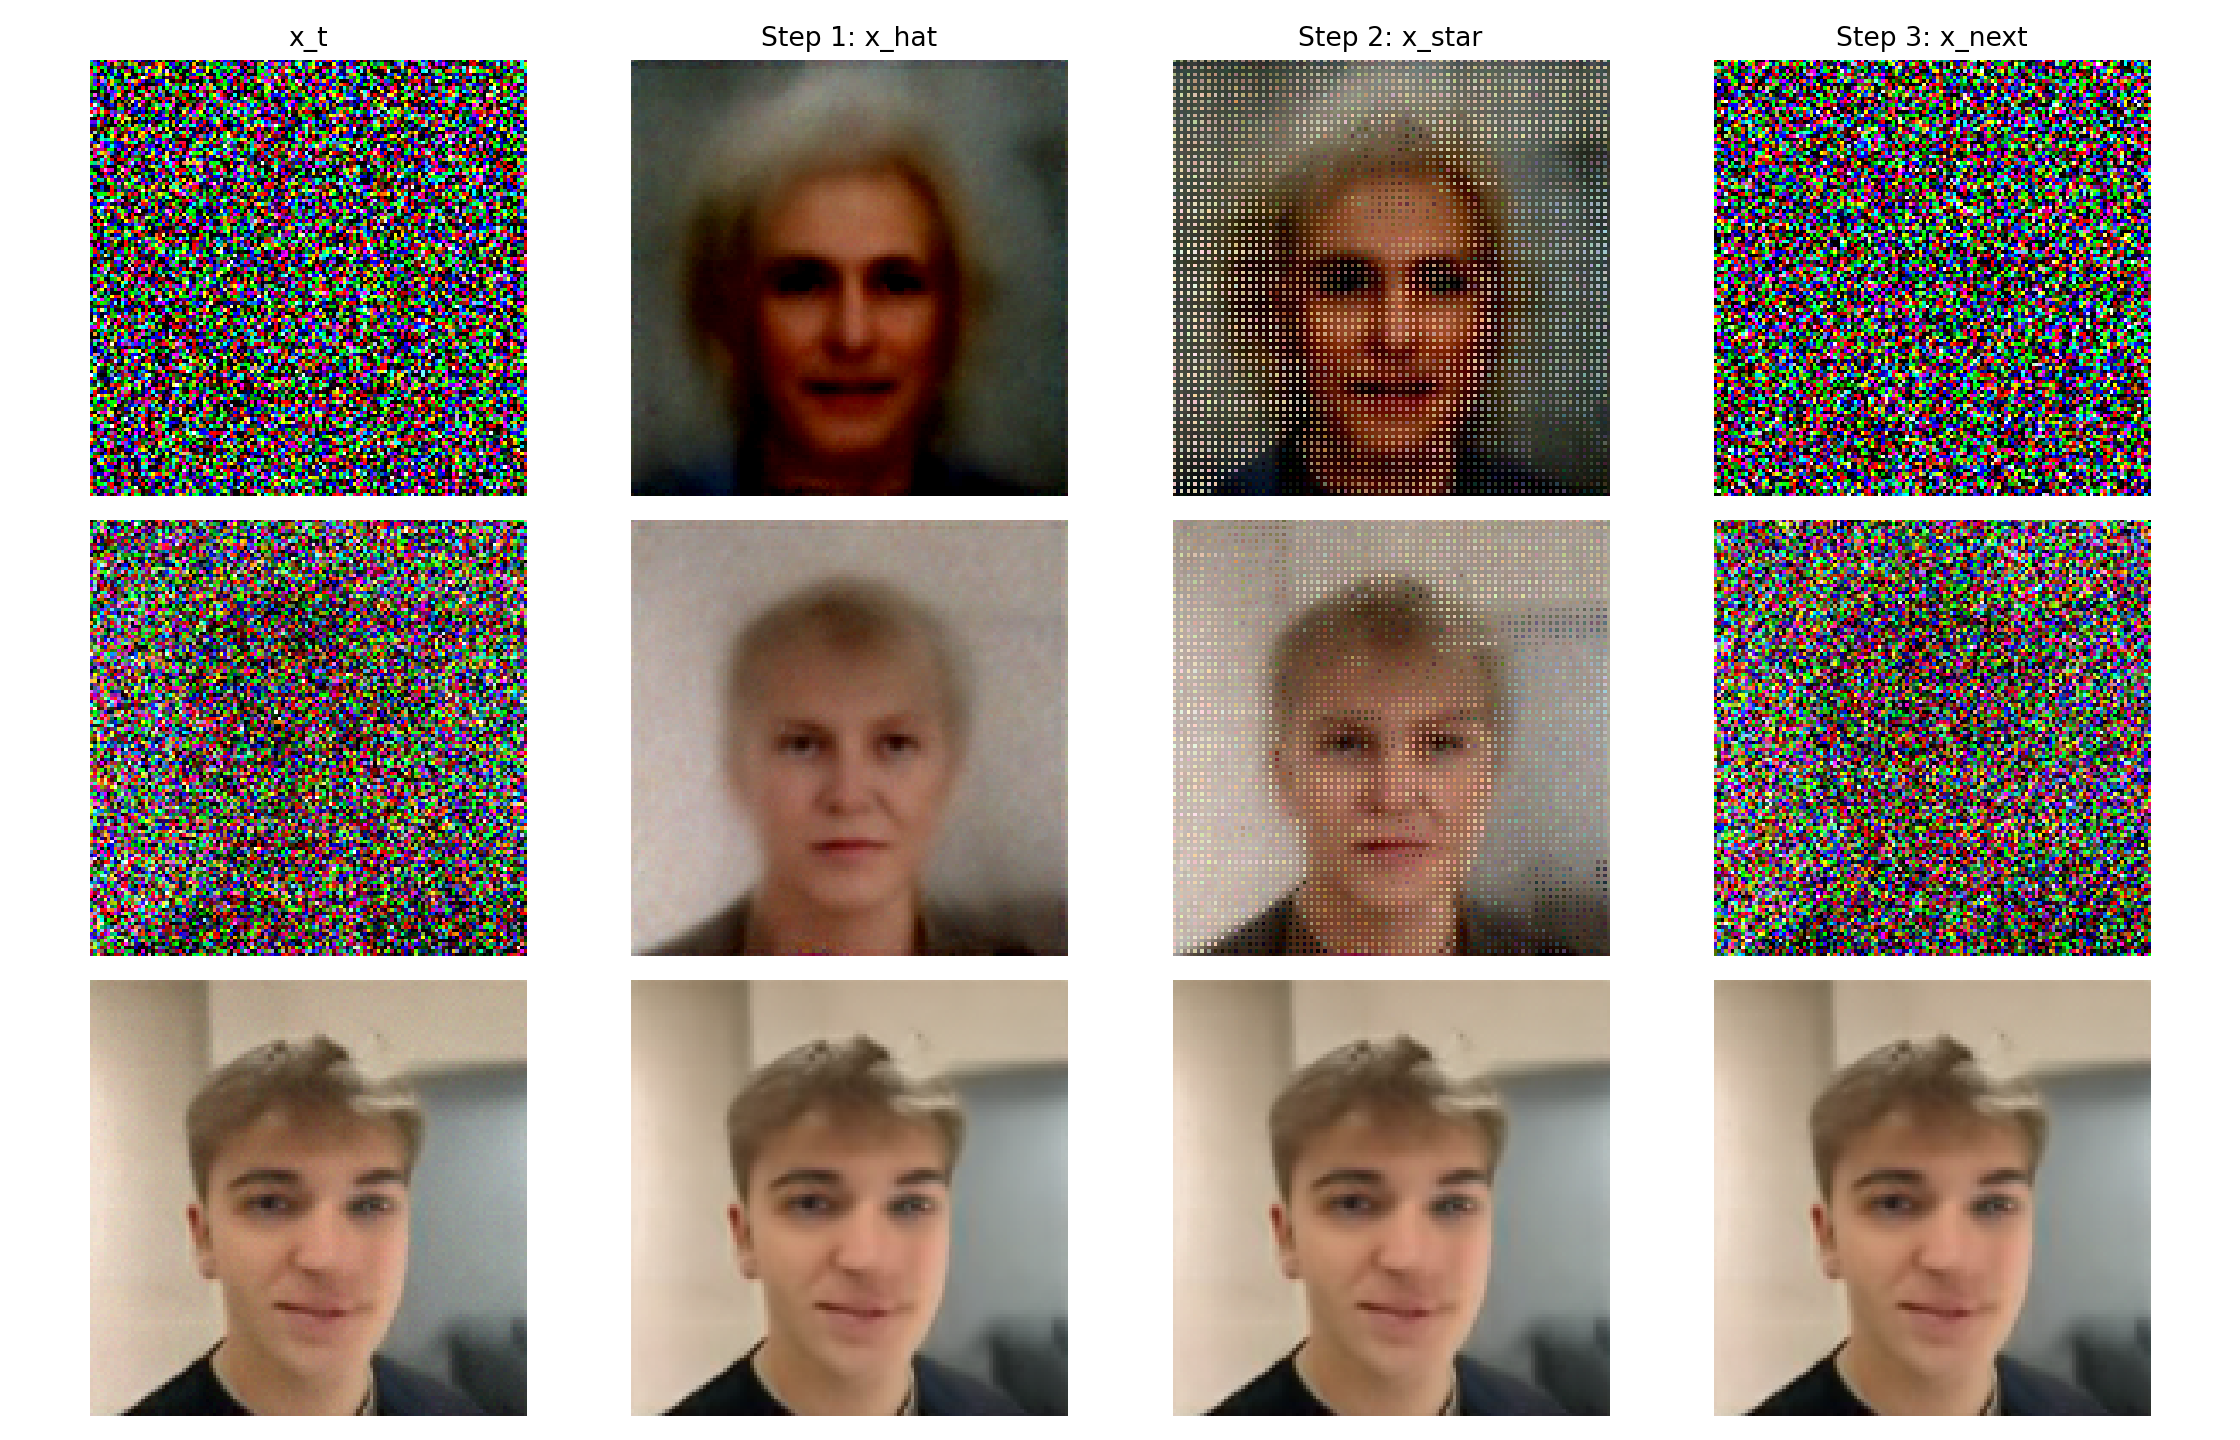
\includegraphics[width=\linewidth]{results_examples/faces/flower_faces_steps.png}
        \caption{Simplified step-by-step view.}
    \end{subfigure}
    \caption{FLOWER reconstruction process for face super-resolution.}
    \label{fig:faces_steps}
\end{figure}

\begin{figure}[H]
    \centering
    \begin{subfigure}[t]{0.49\linewidth}
        \centering
        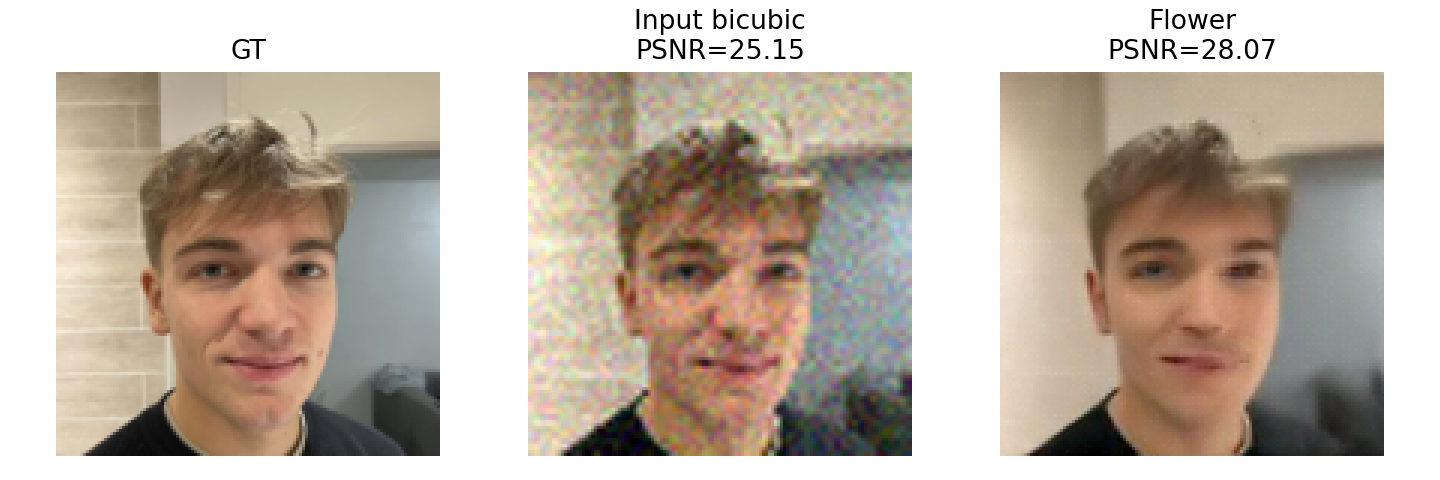
\includegraphics[width=\linewidth]{results_examples/faces/flower_faces_vs_bicubic_examples.png}
        \caption{Standard setting.}
    \end{subfigure}
    \hfill
    \begin{subfigure}[t]{0.49\linewidth}
        \centering
        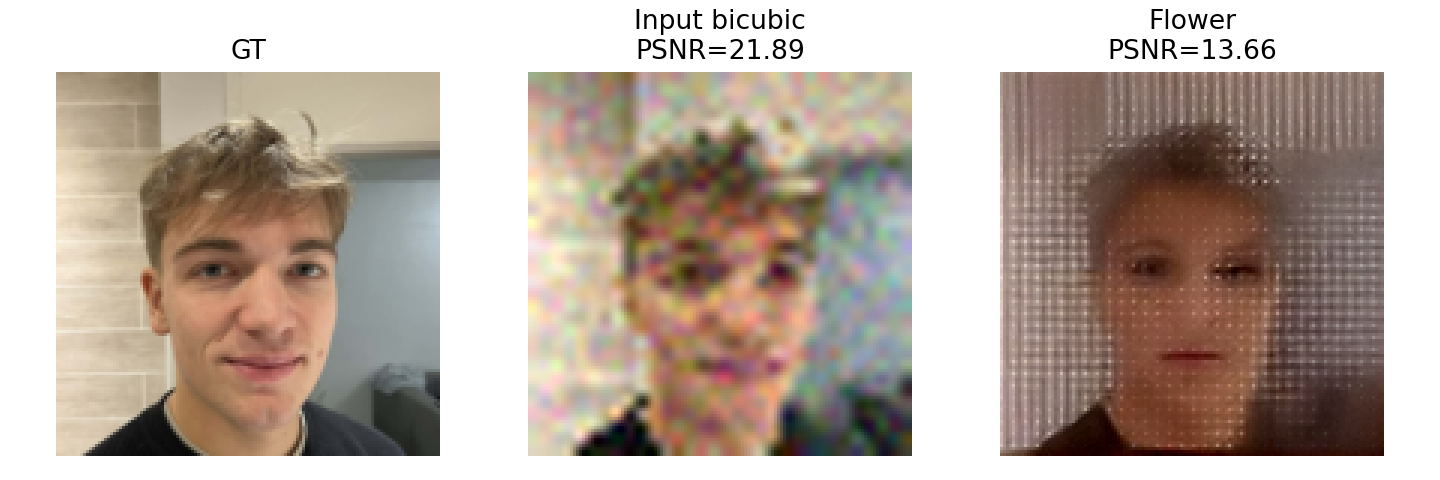
\includegraphics[width=\linewidth]{results_examples/faces/flower_faces_vs_bicubic_examples_hard_sr.png}
        \caption{Hard super-resolution setting.}
    \end{subfigure}
    \caption{Qualitative comparison between bicubic interpolation and FLOWER outputs.}
    \label{fig:faces_compare}
\end{figure}

\noindent
For one representative run of the notebook, we obtain:
\begin{itemize}
    \item Adjoint input: 5.80 dB,
    \item Bicubic interpolation: 25.13 dB,
    \item FLOWER reconstruction: 28.94 dB (gain of +3.81 dB over bicubic).
\end{itemize}
These values are consistent with the visual improvements: FLOWER recovers finer facial details and reduces blur compared to standard interpolation.
\section{Use of Chatbots}
\section{Conclusion}

% ---------------- Appendix ----------------

\newpage
\begin{appendices}

\end{appendices}

\end{document}
